%\pagestyle{fancy}
\chapter{Results}
\label{ch:Results}

\section{Evaluation concept}
\todoin{\begin{itemize}
    \item The straight ramp on floor -2 will be used as main example
    \item All plots will be only made for that ramp
    \item Except maybe for special edge cases (e.g. influence of braking on imu estimation)
    \item All the other ramps will be only evaluated using scores, displayed in tables
\end{itemize}}



\section{Ramp metering? (\glsentrytext{imu})}
\todoin{\begin{itemize}
    \item How well do different \gls{imu} methods work...
    \item ... at ramp detection
    \item ... at ramp distance measuring
    \item ... at angle estimation
\end{itemize}}
\todo[inline, caption={2do}, color=green!40]{
    \begin{minipage}{\textwidth-4pt}
        \begin{itemize}
            \item Which methods should be compared?
            \item Because gravity method only works with odometer, which is only available when driving down or half way up
            \item Should new recording at different offset angles be made?
            \item How to handle false positives, e.g. when braking on level ground?
            \item What to display in the table, only normal drives or also ones with braking etc?
            \item Or evaluate those edge cases separately? (Probably with plot of est angle)
            \item How to handle offline vs live detection (for the offline detection the measurements can be butterworth filtered)?
            \item How to determine the delay of the detection (using the camera image)?
            \item What about the consistency test recordings, how or where to display the results?
        \end{itemize}
    \end{minipage}
}



\section{Ramp detection (\glsentrytext{lidar} and camera)}
\todoin{\begin{itemize}
    \item Confusion matrix or similar (false negatives could be hard (e.g. curve))
    \item Estimated angle and distance compare to ground truth
    \item Do downwards ramp work?
    \item Camera \gls{lidar} projection for nice visualization
    \item Something about camera
\end{itemize}}
\itodo{Make new recordings of level -2 ramps, approaching at different (e.g. 0, 15, 30, 45) angles}

\todo[inline, caption={2do}, color=green!40]{
    \begin{minipage}{\textwidth-4pt}
        \begin{itemize}
            \item Should structure be only one ramp (and direction) or should it include multiple?
            \item How to choose distance interval?
            \item What about offset angle?
            \item What about estimated distance, angle, width and length?
            \item What is a true positive? (E.g. some detected points lie in region, or at least $x$\% lie in region, or less than $y$\% points lie outside\dots)
            \item Are number of frames important?
            \item I've done multiple recordings of e.g. straight ramp on -2 floor, but only one of the ones on floor -1, how to handle?
        \end{itemize}
    \end{minipage}
}
\begin{table}[htbp]
	\centering
	\caption{Performance evaluation}
	\label{tab:eval_table}
	\begin{tabular}[t]{ccccc}
		\toprule
		\textbf{Structure}  & \textbf{Distance}         & \textbf{Frames}   & \textbf{True Positives}   & \textbf{False Positives} \\
		\midrule
		Straight up         & \SIrange{0}{1}{\metre}    & 10                & 100\%	                    & 0\% \\
		Straight down       & \SIrange{10}{15}{\metre}  & 10                & 100\%	                    & 0\% \\
		\bottomrule
	\end{tabular}
\end{table}
% Option1	Structure	Dist interval	TP	FP
% 	Straight up
% 	Straight down
% 	Straight down at 90
% 	Curved up
% 	Curved down

% Option2	Structure	Offset angle	Distance	Frames	TP	FP

% Option3	Structure	StdDev/mean/var etc of distance, angle, width and length


\begin{figure}[htbp]
    \centering
    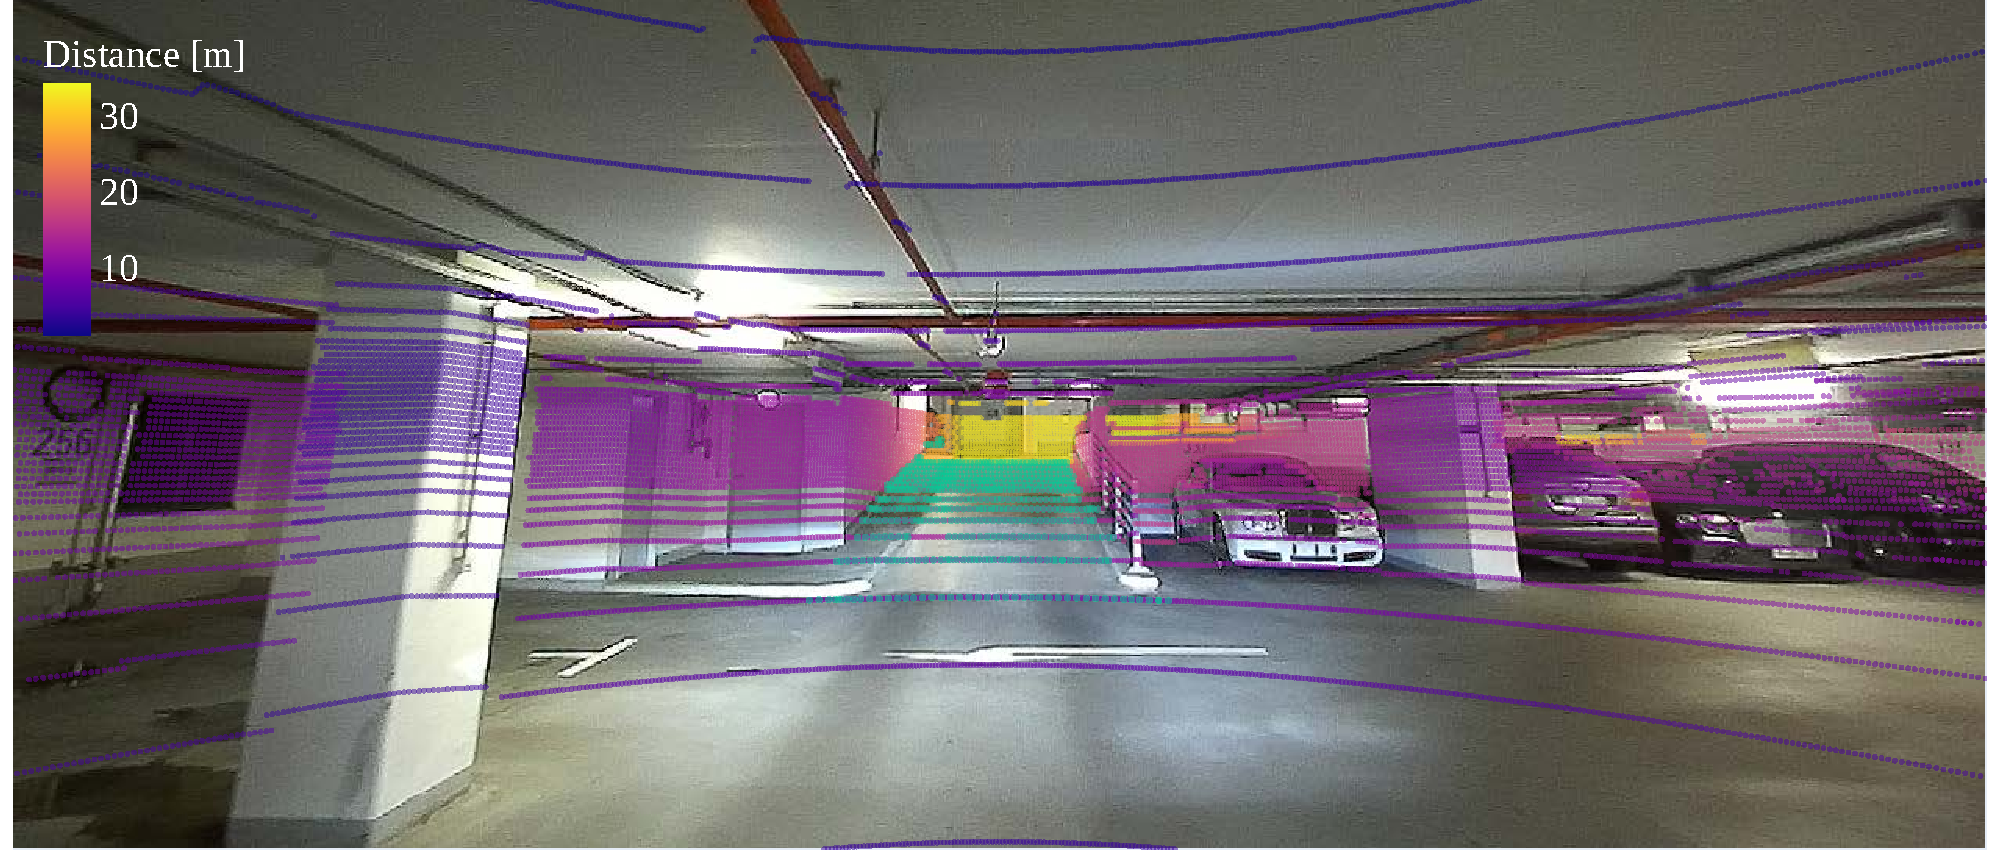
\includegraphics[width=1\linewidth]{points_projection.pdf}
    \caption{Lidar points projected into the camera image. The green points were identified as part of a ramp.}
\end{figure}

\begin{figure}[htbp]
    \centering
    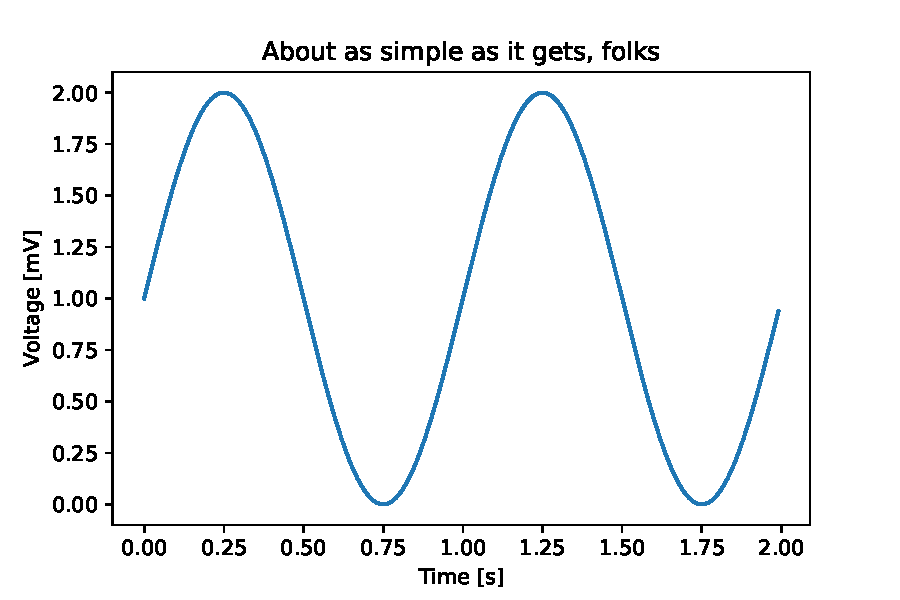
\includegraphics[width=0.7\linewidth]{matplotlib.pdf}
    \caption{Standard matplotlib}
\end{figure}

\begin{figure}[htbp]
    \centering
    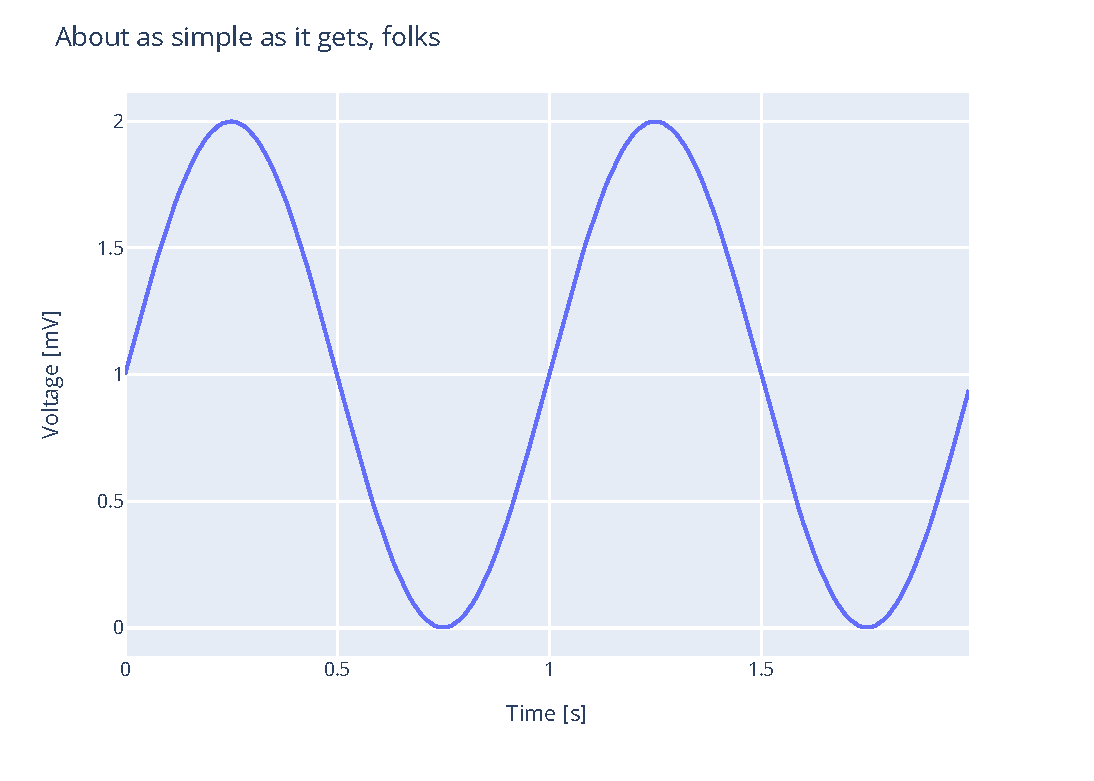
\includegraphics[width=0.7\linewidth]{plotly.pdf}
    \caption{Standard plotly}
\end{figure}